\documentclass{article}	

\usepackage[utf8]{inputenc}
\usepackage{amsmath}
\usepackage[german]{babel}
\usepackage{amssymb}
\usepackage{amsxtra}
\usepackage[dvips]{epsfig,psfrag}
\usepackage{listings}
\usepackage{url}
\usepackage[numbers]{natbib}
\usepackage{hyperref}

\bibliographystyle{plainnat}

\newcommand{\refchapter}[1]{Kapitel~\ref{#1}}
\newcommand{\refsec}[1]{Sektion~\ref{#1}}
\newcommand{\refeqn}[1]{Gleichung~(\ref{#1})}
\newcommand{\reffig}[1]{Abbildung~\ref{#1}}

\title{
{\bf \scriptsize RHEINISCH-WESTF\"ALISCHE TECHNISCHE HOCHSCHULE AACHEN \\
LuFG Informatik 12 (Prof. Dr. rer. nat. Uwe Naumann)}
\vspace{.5cm} \\

\epsfig{file=figures/STCE_Logo_WWW.eps,width=.7\textwidth}
\vspace{1cm} \\
{\bf \Large Korrelation und Regressionsanalyse} \\
{\large Proposal} 
}

\author{vorgelegt von Patrick Neidig (Matr.-Nr. 272582)\\
	und Marius Grysla (Matr.-Nr. 274047)}

\begin{document}

\lstloadlanguages{[ISO]C++}
\lstset{basicstyle=\small, numbers=left, numberstyle=\footnotesize,
  stepnumber=1, numbersep=5pt, breaklines=true, escapeinside={/*@}{@*/}}


\pagestyle{headings}

\maketitle

%\newpage
%\tableofcontents % Brauchen wir für das Proposal ein Inhaltsverzeichnis?

\newpage

%TODO: Merkmal vs. Variable?
%TODO: Schreibweise: Nag C Biliothek

\section{Einleitung}
Im Rahmen dieser Arbeit werden wir uns mit den Funktionen beschäftigen, welche die {\it NAG C Library}, eine Sammlung numerischer Algorithmen der {\it Numerical Algorithms Group} für die Programmiersprache {\it C}/{\it C++}, ihren Anwendern zur {\it Korrelation} und zur {\it Regressionsanalyse} zur Verfügung stellt.\\
Die Begriffe "`Korrelation"' und "`Regressionsanalyse"' sind der {\it deskriptiven Statistik} zuzuordnen, welche sich mit der Beschreibung und Darstellung von Daten befasst, die zuvor durch Erhebungen (z.B. Befragungen) oder Experimente gewonnen wurden.\\
Ein Beispiel für eine Erhebung wäre etwa die Studentische Lehrveranstaltungsbewertung, die an der {\it RWTH Aachen} regelmäßig durchgeführt wird. Die bei Erhebungen und Experimenten gewonnenen Daten umfassen {\it Merkmale} bestimmter {\it Merkmalsträger}: In unserem Beispiel wären die Merkmalsträger unter anderem die Studenten, die an der jeweiligen Erhebung teilnehmen, da sie zu mehreren persönlichen Merkmale befragt werden -- nämlich zu ihrem Geschlecht, ihrem Fachsemester und ihrer Nationalität. Weitere Merkmalsträger sind selbstverständlich die Lehrveranstaltung, der Dozent sowie die Rahmenbedingungen, deren unterschiedliche Merkmale von den Studenten bewertet werden. Die einzelnen Merkmale können verschiedene {\it Merkmalsausprägungen} annehmen: Das Merkmal "`Fachsemester"' eines Studenten kann bspw. die Ausprägungen "`1-2"', "`3-4"', ..., "`9-10"' oder "`über 10"' annehmen. Die Merkmale der Lehrveranstaltung und des Dozenten können von den Studenten überwiegend auf einer fünfstufigen Skala von "`trifft völlig zu"' bis "`trifft nicht zu"' oder mit Noten von "`sehr gut"' bis "`mangelhaft"' bewertet werden, wodurch sie eben diese möglichen Ausprägungen erhalten.\\
Im Anschluss an eine Erhebung oder ein Experiment lässt sich  der jeweils gewonnene Datensatz wie bereits erwähnt mit Hilfe der deskriptiven Statistik auf unterschiedliche Art und Weise beschreiben und darstellen. Eine Möglichkeit ist es, ein einzelnes Merkmal zu betrachten und z.B. den Mittelwert der Noten zu berechnen, welche die Studenten der Lehrveranstaltung gegeben haben. Dies ist das Feld der {\it univariaten Statistik}. Eine weitere Möglichkeit ist es, zwei oder mehrere Merkmale gleichzeitig zu betrachten, um sie auf eventuelle Zusammenhänge zu prüfen. Es wäre bspw. denkbar, dass das Merkmal "Fachsemester" eines Studenten und seine Bewertung des Merkmals "Schwierigkeitsgrad" der Lehrveranstaltung auf gewisse Weise zusammenhängen, was wichtig für die Interpretation des letzteren Merkmals wäre. Dies ist das Feld der {\it bi-} bzw. {\it multivariaten Statistik}. Hier sind schließlich auch die Korrelation und die Regressionsanalyse einzuordnen, welche sich beide mit der Beschreibung zweier oder mehrerer Merkmale und ihres Zusammenhangs beschäftigen. Wir werden uns in dieser Arbeit hauptsächlich auf die gleichzeitige Betrachtung zweier Merkmale beschränken, da eine Verallgemeinerung auf mehrere Merkmale ihren Rahmen sprengen würde.
%TODO: Mehrere unabhängige Variablen sollen nicht möglich sein?

\subsection{Motivation}

Es ist natürlich nicht nur im Rahmen der Studentischen Lehrveranstaltungsbewertung an der RWTH Aachen interessant, die möglichen Zusammenhänge von Merkmalen festzustellen. Die Anwendungsbereiche der Korrelation und der Regressionanalyse erstrecken sich von der Wirtschaft (Wie wirken sich Werbemaßnahmen auf die Verkaufszahlen eines Produkts aus?) über die Medizin (Durch welche genetischen Veranlagungen wird eine Krankheit begünstigt?) bis hin zu Sozial- und Naturwissenschaften, um nur einige Beispiele zu nennen. Auf Grund der vielfachen Anwendung ist es wünschenswert und oft sogar nötig (etwa bei sehr großen Datensätzen), solche statistischen Berechnungen automatisiert ausführen zu lassen. Die {\it NAG C Library} ist dabei ein wichtiges Hilfsmittel, stellt sie doch viele der nötigen Funktionen bereits in fertiger Form zur Verfügung, so dass sie in beliebige Anwendungsprogramme integriert werden können -- vorausgesetzt, sie wurden in{\it C}/{\it C++} oder einer anderen unterstützten Programmiersprache geschrieben.

\section{Korrelation}

Der Begriff {\it Korrelation} bezeichnet einen Zusammenhang zwischen zwei oder mehreren Merkmalen. Man sagt auch, dass diese Merkmale {\it korrelieren}. Wie stark dieser Zusammenhang ist, lässt sich messen, indem man verschiedene sog. {\it Korrelationskoeffizienten} berechnet. Im Folgenden werden wir zwei dieser Korrelationskoeffizienten vorstellen und im weiteren Verlauf der Arbeit näher untersuchen, wie ihre Berechnung in den entsprechenden Funktionen der {\it NAG C Library} implementiert ist.

\subsection{Korrelationskoeffizient nach Bravais und Pearson}

Der Korrelationskoeffizient $r$ nach Bravais und Pearson (auch {\it empirischer Korrelationskoeffizient} oder {\it Produkt-Moment-Korrelation} genannt) misst die Stärke des \underline{linearen} Zusammenhangs zweier Merkmale $X$ und $Y$ mit den Merkmalsausprägungen $x_1,x_2,...,x_n$ bzw. $y_1,y_2,...,y_n$ und ist definiert als
\begin{equation*}
    r=\dfrac{s_{XY}}{s_Xs_Y}=\dfrac{\sum_{i=1}^{n}{(x_i-\bar{x})(y_i-\bar{y})}}{\sqrt{\sum_{i=1}^{n}{(x_i-\bar{x})^2\sum_{i=1}^{n}{(y_i-\bar{y})^2}}}},\\
\end{equation*}
wobei $s_{XY}\) für die {\it Kovarianz} der Merkmale $X\) und $Y$ steht sowie $s_{X}$ bzw.  $s_{Y}$ für ihre jeweiligen {\it Standardabweichungen}. Dabei ist zusätzlich anzumerken, dass beide Merkmale mindestens in {\it intervallskalierter} Form vorliegen müssen, d.h. alle möglichen Merkmalsausprägungen müssen als Zahlen interpretierbar sein, deren Abstände genau messbar sind.\\
Der Wertebereich von $r$ ist $-1 \leq r \leq +1$. Der für zwei Merkmale berechnete Wert von $r$ ist folgendermaßen zu interpretieren:
\begin{itemize}
    \item $r>0$: Positive Korrelation: Es besteht ein gleichsinniger linearer Zusammenhang zwischen den Merkmalen, d.h. alle Paare $(x_i, y_i)$ mit $i=1,...,n$ der Merkmalsausprägungen bilden annähernd eine Gerade mit positiver Steigung.
    \item $r<0$: Negative Korrelation: Es besteht ein gegensinniger linearer Zusammenhang zwischen den Merkmalen, d.h. alle Paare bilden annähernd eine Gerade mit negativer Steigung.
    \item $r=0$: Keine Korrelation: Es besteht kein linearer Zusammenhang und somit keine Korrelation zwischen den Merkmalen.
\end{itemize}
In der {\it NAG C Library} dient die Funktion nag\_corr\_cov zur Berechnung dieses Korrelationskoeffizienten.\\
Liegen die Merkmale, deren Korrelationsstärke gemessen werden soll, nur in {\it ordinalskalierter} Form vor, d.h. sind alle möglichen Merkmalsausprägungen lediglich nach einer Reihenfolge sortierte Kategorien, kann auf den folgenden Korrelationskoeffizienten zurückgegriffen werden.

\subsection{Rangkorrelationskoeffizient nach Spearman}

Der Rangkorrelationskoeffizient $r_{SP}$ nach Spearman misst die Stärke des \underline{mono-}\\\underline{tonen} Zusammenhangs zweier mindestens ordinalskalierter Merkmale, indem die ursprünglichen $x$- und $y$-Merkmalsausprägungen vor der eigentlichen Berechnung in {\it Ränge} transformiert werden.\\
Dabei wird jedem $x_i$ mit $i=1,...,n$ als Rang die Zahl der Position zugewiesen, die $x_i$ erhält, wenn man $x_1, x_2, ..., x_n$ der Größe nach anordnet. Für die so geordneten Merkmalsausprägungen $x_{(1)}<x_{(2)}<...<x_{(n)}$ gilt dann $rg(x_{(i)})=i$. Analog wird unabhängig von den $x$-Werten auch mit den $y$-Werten verfahren. Somit ergeben sich aus den ursprünglichen Paaren $(x_i, y_i)$ neue Rangpaare $(rg(x_i), rg(y_i))$ mit $i=1,...,n$.\\
Treten $x$- oder $y$-Merkmalsausprägungen doppelt auf, ist die Rangvergabe nicht eindeutig. In einem solchen Fall werden deshalb {\it Durchschnittsränge} gebildet, d.h. jeder der betroffenen Merkmalsausprägungen wird als Rang der arithmetische Mittelwert der potentiellen Ränge zugewiesen. Ein Beispiel: In einem Datensatz liegen drei gleiche Merkmalsausprägungen vor, welche die Ränge 5, 6 und 7 belegen könnten. Weil sie jedoch nicht eindeutig der Größe nach angeordnet werden können, erhalten alle drei den Durchschnittsrang $rg=(5+6+7):3=6$.\\
Der eigentliche Rangkorrelationseffizient wird schließlich berechnet, indem der Korrelationskoeffizient nach Bravais und Pearson auf die transformierten Rangpaare $(rg(x_i), rg(y_i))$ mit $i=1,...,n$ angewendet wird. Er ist somit definiert als
\begin{equation*}
    r_{SP}=\dfrac{\sum_{i=1}^{n}{(rg(x_i)-\bar{rg}_X)(rg(y_i)-\bar{rg}_Y)}}{\sqrt{\sum_{i=1}^{n}{(rg(x_i)-\bar{rg}_X)^2\sum_{i=1}^{n}{(rg(y_i)-\bar{rg}_Y)^2}}}},\\
\end{equation*}
wobei $\bar{rg}_X$ und $\bar{rg}_Y$ für die Mittelwerte aller Ränge des Merkmals $X$ bzw. $Y$ stehen. Der Wertebereich von $r_{SP}$ ist entsprechend gleich dem Wertebereich vom $r$ und der berechnete Wert analog für den monotonen Zusammenhang zu interpretieren.
In der {\it NAG C Library} dient die Funktion nag\_ken\_spe\_corr\_coeff zur Berechnung dieses Korrelationskoeffizienten.

\subsection{Weiterführende Berechnungen}

Liegt eine Korrelation zwischen zwei Merkmalen vor, ist damit nicht bewiesen, dass auch ein \underline{kausaler} Zusammenhang vorliegt. Das Phänomen der sog. {\it Scheinkorrelation} besagt, dass eine Korrelation zwischen den Merkmale $X$ und $Y$ (z.B. Körpergröße und Wortschatz von Kindern) unter Umständen auf den Einfluss eines weiteren Merkmals $Z$ (z.B. Alter) zurückgeführt werden kann. Dies kann durch die Berechnung der partiellen Korrelation überprüft werden, wozu in der {\it NAG C Library} die Funktion nag\_partial\_corr dient. Diese und ggf. weitere Funktionen werden wir ebenfalls näher betrachten, sofern es der Rahmen dieser Arbeit erlaubt.

\section{Regressionsanalyse}

Der zweite große Teil der Arbeit wird sich mit der Regressionsanalyse beschäftigen.
Mittels dieser wird wieder, wie bei der Korrelation, die Beziehung einer abhängigen Variable zu einer oder mehreren unabhängigen Variablen untersucht.
Allerdings wird nun versucht, diesen Zusammenhang graphisch durch das fitten einer Kurve an den gemessenen Datensatz zu erreichen.

Die NAG-Bibliothek bietet dazu zahlreiche Funktionen, von verschiedenen Regressionsarten bis hin zu Hilfen für die Bewertung und Validierung von Regressionsmodellen, die nun kurz vorgestellt werden.
Für die theoretischen Grundlagen wurden \cite{Cramer2007} und \cite{Fahrmeier2010} zusammen mit der Einführung der NAG-Bibliothek (\cite{nag:intro}) verwendet.

\subsection{Regressionsmodelle}

Der einfachste Ansatz für eine Regression ist die lineare Regression mit einer unabhängigen Variablen.
Dabei wird versucht eine lineare Funktion zu finden die die zuvor gemessene Daten möglichst gut annähert, die sog. "`Ausgleichsgerade"'.
Der Ansatz dazu ist
\begin{equation*}
 Y = \alpha + \beta X +\epsilon
\end{equation*}
wobei $X$ und $Y$ metrisch skalierte Merkmale sind und $\epsilon$ ein Fehler, der nicht durch $X$ erklärt werden kann.
%TODO: Methode kleinster Quadrate
In der NAG-Bibliothek wird diese Funktionalität durch die Funktion nag\_simple\_linear\_regression zur Verfügung gestellt.

Der Schwerpunkt in der Regressionsanalyse soll bei dieser Arbeit allerdings auf der lineare Mehrfachregression (nag\_regsn\_mult\_linear) liegen.
Diese ermöglicht es mehr als nur ein erklärendes Merkmal in die Regression mit einzubeziehen und ist somit eine Verallgemeinerung der einfachen Regression.
Dabei sind auch verschieden skalierte Regressanden möglich (zB. metrisch und binär skaliert), was in der Arbeit durch ein Beispiel verdeutlicht werden soll.

Weiterhin soll die robuste Regression (nag\_robust\_m\_regsn\_user\_fn) in der Arbeit behandelt werden, insofern der Platz ausreicht.
Ihr Ziel ist es, extremen Beobachtungen weniger Einfluss auf die Regression zu geben.
Dies kann vor allem bei Meßdaten von Vorteil sein, da sich Meßfehler somit nicht so stark auf die Regression auswirken.
Als theoretische Grundlage sollen hier die Bücher \cite{Hampel1986} und \cite{Huber1981} dienen.


\subsection{Analyse}

Zusätzlich zu der Berechnung der verschieden Regressionsmodelle bietet die NAG-Bibliothek auch Funktionen zur Auswahl des Regressionsmodells und zur Modellvalidierung.

Für die Auswahl des Modells sollen in der Arbeit zwei Metriken behandelt werden: Die Residualstreuung und das Bestimmtheitsmaß $\mathcal{R}^2$.
Beide können uns eine Idee davon geben, wie gut die unabhängigen Variablen die Werte der abhängigen Variablen erklären können.
Die Residualstreuung gibt die Verteilung der Differenzen zwischen der angenäherten Funktion und den wirklichen Daten an.
Sollte sie unregelmäßig sein (wenn die Residuen beispielsweise mit einer Variablen anwachsen) ist dies ein starkes Indiz dafür, dass ein zu simples Modell gewählt wurde. 
Das Bestimmtheitsmaß gibt dagegen an, wie gut abhängige Variable durch die Regression erklärt werden kann.
Berechnet werden kann es auch durch eine Quadrierung des Bravais-Pearson Korrelationskoeffizienten, was den starken Zusammenhang von Korrelation und Regressionsanalyse zeigt.

Für die Modellvalidierung stehen verschiedene Werkzeuge zur Verfügung, welche bei der Bewertung der Güte der Regression und deren Verbesserung genutzt werden können.
In diese Kategorie fallen zum Beispiel der Cooks-Abstand (ermittelt besonders einflußreiche Punkte), die T-Statistik (Testet, ob eine unabhängige Variable für die Regression wichtig ist) oder der Durbin-Watson-Test (Ermittelt, ob die Residuen von den zuvor gemessenen Werten abhängig sind.
In der Ausarbeitung werden diese allerdings aus Platzgründen nicht behandelt werden.

\section{Leistungsanalyse}

Die zwei wichtigsten Qualitätskriterien für mathematischen Funktionen sind Korrektheit und der Verbrauch von Ressourcen.
Eine gute Funktion sollte daher für alle möglichen Parameter den mathematisch korrekten Wert berechnen und dies zudem mit möglichst wenig Ressourcen, wie Speicher oder Prozessor-Laufzeit.
Da die NAG C-Bibliothek bereits seit 1990 entwickelt wird\cite{Wikipedia:nag} und zudem alle Methoden vor der Veröffentlichung auf Korrektheit geprüft werden\cite{NAG2011}, ist nicht davon auszugehen, dass Fehler vorhanden sind.
Daher wird in der Ausarbeitung nur die Leistung behandelt.

Dazu sollen zwei Algorithmen der Bibliothek auf ihren Ressourcenverbrauch untersucht werden: Der Bravais-Pearson Korrelationskoeffizient und die multiple lineare Regression.
Für beide werden Laufzeit und Speicherverbrauch unter Benutzung von verschiedenen Parametern mit ansteigender Komplexität untersucht.
Damit alle Berechnungen vergleichbar sind, werden sie auf dem RWTH Cluster ausgeführt.

\section{Zeitplan}

Der Zeitplan für die Seminararbeit und die verschiedenen Präsentationen richtet sich hauptsächlich nach den vorgegebenen Terminen.
Eine Übersicht über die Arbeitsschritte wird in Abbildung \ref{fig:Zeitplan} gezeigt.
\begin{figure}[t]
 %TODO: Bild verkleinern?
 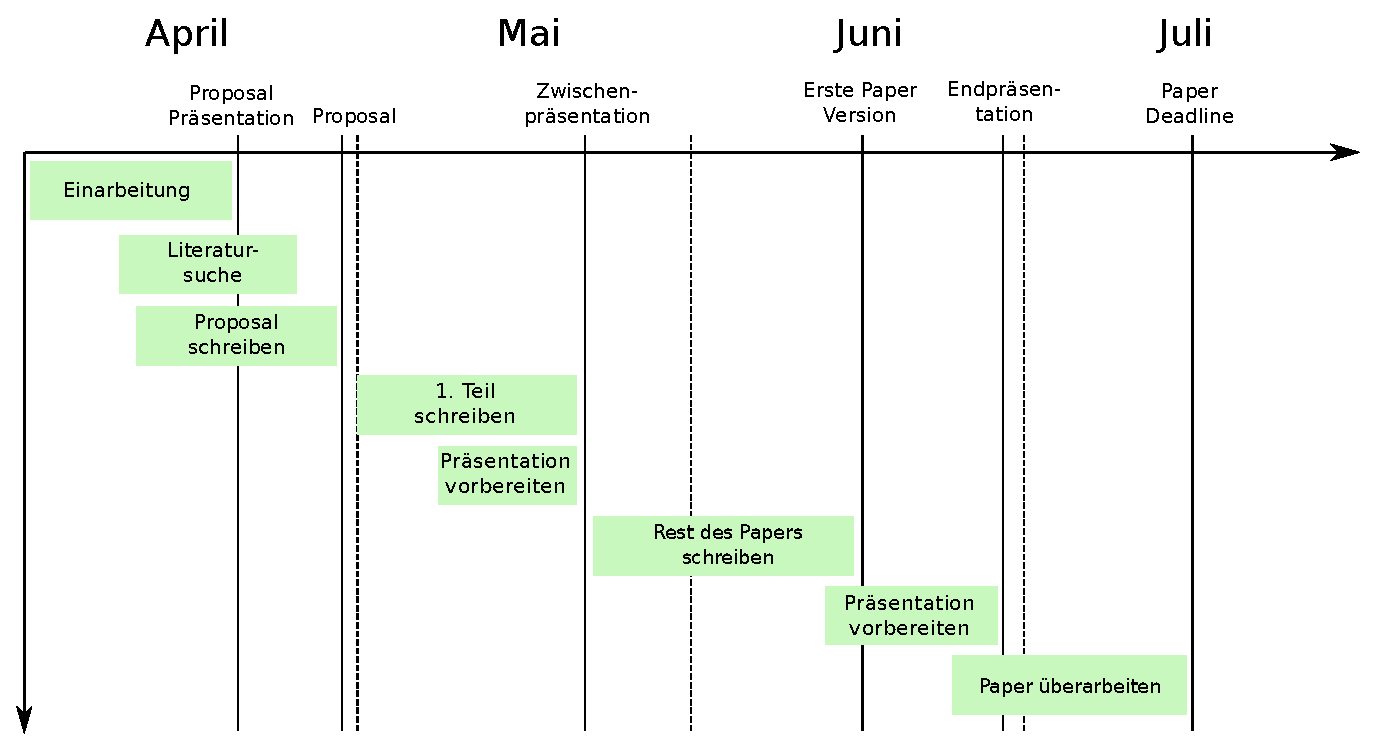
\includegraphics[width=\linewidth]{./figures/Workplan-adj-small.eps}
 \caption{Der geplante Arbeitsverlauf mit Abgabezeitpunkten.}
 \label{fig:Zeitplan} 
\end{figure}
Auf der x-Achse ist dabei der Zeitverlauf und auf der y-Achse die Arbeitsschritte abgebildet.

Der erste Teil besteht aus der Einarbeitung in die statistischen Grundlagen, sowie in die verfügbaren Funktionen der Bibliothek.
Darauf folgt eine Literatursuche, deren Fokus auf auf den mathematischen Funktionen hinter den NAG-Funktionen liegt.
Nach der Abgabe dieses Proposals werden wir mit dem Schreiben des ersten Teils der Arbeit beginnen. 
%TODO: @Patrick: Ist das richtig so?
Dieser soll neben der Einleitung aus der Behandlung von jeweils einer Funktion für Korrelation und Regression bestehen, welche dann auch in der Zwischenpräsentation vorgestellt werden.
Bis zum ersten Abgabetermin Mitte Juni wird die Ausarbeitung dann noch um weitere Algorithmen und eine Laufzeitanalyse erweitert.
%TODO: Was wird noch in der Hauptpräsentation vorgestellt?
In der letzten Präsentation werden die Ergebnisse der Analyse präsentiert und außerdem wird die Benutzung der Bibliothek anhand eines größeren Beispiels demonstriert.
Zuletzt soll die Ausarbeitung noch einmal überarbeitet und Fehler korrigiert werden.

Da wir da Thema nur zu zweit bearbeiten ist kein wirklicher Notfallplan vorgesehen. 
Falls das Seminar von einem Teammitglied abgebrochen wird, werden die Grundlagen vom jeweils Anderen übernommen, der dafür seinen Themenbereich entsprechend kürzer behandelt.

%TODO: Bibtex Einträge sollten auf Deutsch sein (``und'' statt ``and'')
\bibliography{report}


\end{document}
